\begin{recipe}
    [% 
        preparationtime = {\unit[30]{min}},
        bakingtime = {\unit[1]{h}},
        portion = {\portion{4}}
    ]
    {Curry with sweet potatoes and butternut squash}

    \setRecipeLengths{
        ingredientswidth=6cm
    }
    \ingredients[15]{%
        1 & Onion \\
        1 & Sweet potato \\
        1 & Butternut squash \\
        2 can & Tomatoes \\
        \unit[2]{c.} & Kale \\
        1-2 cans & Chickpea \\
        1 can & Coconut milk \\
        & \\
        & Curry powder \\
        & Turmeric \\
        & Coriander \\
        & Cumin \\
        & Garam Masala \\
        & Cinnamon \\
        & Cloves
    }

    \preparation{%
        \step Dice onion, chop up sweet potato and butternut squash.

        \step  Fry onion with spices.
        Add canned tomatoes and veg apart for kale.
        Simmer for about an hour.

        \step Add kale, chickpea and coconut milk, keep heating for 5 min.
    }


    \hint{%
        Butternut squash can be swapped for carrots, kale for spinach and chickpea for other pulses.
    }
\end{recipe}

\begin{figure}[h]
    \centering
    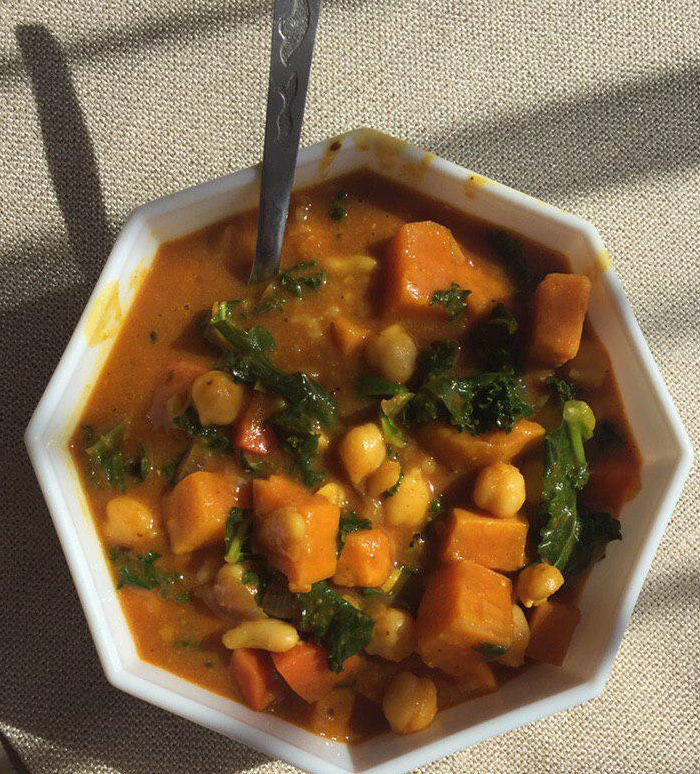
\includegraphics[width=12cm]{pic/curry_sweet_potato}
\end{figure}
